% The document class supplies options to control rendering of some standard
% features in the result.  The goal is for uniform style, so some attention 
% to detail is *vital* with all fields.  Each field (i.e., text inside the
% curly braces below, so the MEng text inside {MEng} for instance) should 
% take into account the following:
%
% - author name       should be formatted as "FirstName LastName"
%   (not "Initial LastName" for example),
% - supervisor name   should be formatted as "Title FirstName LastName"
%   (where Title is "Dr." or "Prof." for example),
% - degree programme  should be "BSc", "MEng", "MSci", "MSc" or "PhD",
% - dissertation title should be correctly capitalised (plus you can have
%   an optional sub-title if appropriate, or leave this field blank),
% - dissertation type should be formatted as one of the following:
%   * for the MEng degree programme either "enterprise" or "research" to
%     reflect the stream,
%   * for the MSc  degree programme "$X/Y/Z$" for a project deemed to be
%     X%, Y% and Z% of type I, II and III.
% - year              should be formatted as a 4-digit year of submission
%   (so 2014 rather than the accademic year, say 2013/14 say).

\documentclass[ % the name of the author
                    author={Student name},
                % the name of the supervisor
                supervisor={Supervisor name},
                % the degree programme
                    degree={BSc},
                % the dissertation    title (which cannot be blank)
                     title={Title},
                % the dissertation subtitle (which can    be blank)
                  subtitle={},
                % the dissertation     type
                %  type={enterprise},
                % the year of submission
                      year={2019} ]{dissertation}

\usepackage{opera}
\begin{document}

% =============================================================================

% This section simply introduces the structural guidelines.  It can clearly
% be deleted (or commented out) if you use the file as a template for your
% own dissertation: everything following it is in the correct order to use 
% as is.

\iffalse
\section*{Prelude}
\thispagestyle{empty}

A typical dissertation will be structured according to (somewhat) standard 
sections, described in what follows.  However, it is hard and perhaps even 
counter-productive to generalise: the goal is {\em not} to be prescriptive, 
but simply to act as a guideline.  In particular, each page count given is
important but {\em not} absolute: their aim is simply to highlight that a 
clear, concise description is better than a rambling alternative that makes
it hard to separate important content and facts from trivia.

You can use this document as a \LaTeX-based~\cite{latexbook1,latexbook2} 
template for your own dissertation by simply deleting extraneous sections
and content; keep in mind that the associated {\tt Makefile} could be of
use, in particular because it automatically executes \mbox{BibTeX} to 
deal with the associated bibliography.  

You can, on the other hand, opt {\em not} to use this template; this is a 
perfectly acceptable approach.  Note that a standard cover and declaration 
of authorship may still be produced online via
\[
\mbox{\url{http://www.cs.bris.ac.uk/Teaching/Resources/cover.html}}
\]

\fi
% =============================================================================

% This macro creates the standard UoB title page by using information drawn
% from the document class (meaning it is vital you select the correct degree 
% title and so on).

\maketitle

% After the title page (which is a special case in that it is not numbered)
% comes the front matter or preliminaries; this macro signals the start of
% such content, meaning the pages are numbered with Roman numerals.

\frontmatter

% This macro creates the standard UoB declaration; on the printed hard-copy,
% this must be physically signed by the author in the space indicated.

\makedecl

\chapter*{Abstract}

A short abstract (\ie less than a page).


\chapter*{Acknowledgements}

A place to thank everyone for their help (family, friend, supervisors, tutors \etc). Keep it short again (\ie less than a page).

% LaTeX automatically generates a table of contents, plus associated lists 
% of figures, tables and algorithms.  The former is a compulsory part of the
% dissertation, but if you do not require the latter they can be suppressed
% by simply commenting out the associated macro.

\tableofcontents

\listoffigures

\listoftables

\mainmatter


\chapter{Introduction}
\label{chap:introduction}
\section{Some section}
\label{chap:introduction:somesec}

This is a citation~\cite{smalley2001implementing}.

\begin{table}[h]
	\centering
	\begin{tabular}{|l|l|}
		A* & A \\
		\hline
		1  & 2
	\end{tabular}
	\caption{A super interesting table.}
	\label{table:superinteresting}
\end{table}

I can describe the data shown in \autoref{table:superinteresting}.

\section{And another}
\label{chap:introduction:another}

\begin{figure}[h]
	\centering
	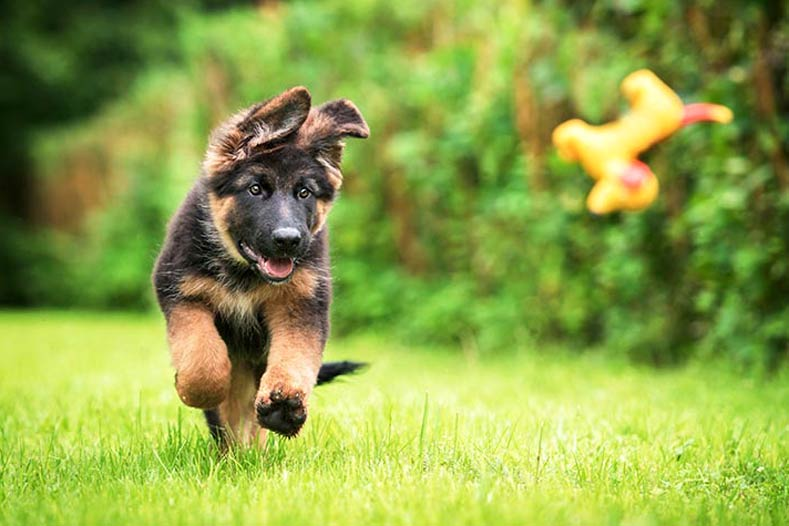
\includegraphics[width=\textwidth]{./img/puppy.jpg}
	\caption{A cute puppy.}
	\label{image:puppy}
\end{figure}

\autoref{image:puppy} show a very cute puppy.

\notespv{can put comments!}

\notestd{and the student can respond!}


\bibliography{biblio}

\backmatter
\appendix

\chapter{My First Appendix}
\label{appendix:first}
I can give more information about \autoref{image:puppy} that appeared in \autoref{chap:introduction}.

\chapter{And a second one}

\end{document}
